% !TEX root =../thesis-letomes.tex

\chapter{Software Engineering}

The project has been defined by a relatively wide scope of disciplines that we have worked on. Mathematic derivations, astrophysics intuition, machine learning, high-performance computing, and software engineering. The last of those particularly because of the simultaneous need for rapid prototyping and strong performance characteristics. Essentially, we needed to be able to test a plethora of different ideas to answer all our questions, but since the computations are so relatively expensive, we wanted to build a few solid modules that could be treated as black boxes for our overarching purposes. Essentially, we rewrote the simulator from the precursor project from the ground up, with a focus on modularity and extensibility. This was done on basis of the model inherent in the original, to give us a consistent "ground truth" with which to compare our new simulator.


\section{Software Architecture Overview}
Our system is organized as two general spheres with an interface between them. One sphere is the ES algorithm and its various auxiliary functions, and the other is the orbsim module, which takes care of the astrophysics aspect; turning launch parameters into trajectories. Between them is an interface that turns machine learning parameters into astrophysics parameters, and the reverse. Visualized in \cref{fig:software_architecture}, this architecture lets us keep variable names consistent with the literature for both domains. The multidisciplinary nature of this project and its authors made this a boon.

\begin{figure}
    \centering
    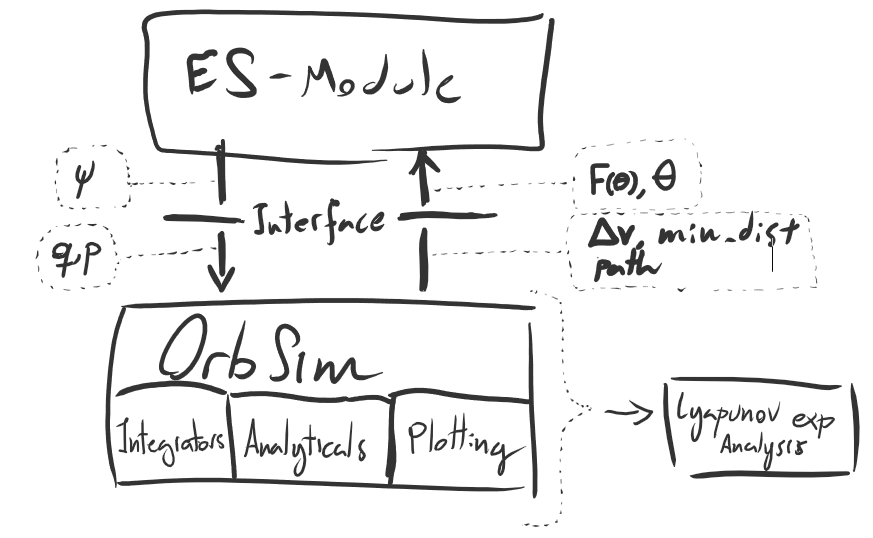
\includegraphics[width=\linewidth]{fig/software_architecture}
    \caption{The architecture of the project, ES module inputs parameters to orbital simulator, which returns scores and trajectories. Not pictured are the many auxiliary analysis scripts which also use orbsim}
    \label{fig:software_architecture}
\end{figure}

\section{Legacy Software from BSc Project}
\section{Unit Testing}
ensuring correctness of complex system with many edits taking place.
\section{Software Architecture}
\subsection{Orbsim Module}
We have arranged our code into a python module that offers us some nice modularity and extensibility, at least within the bounds of our relatively specific problem. What follows is an explanation of the architecture of this module.

We packaged the new simulator into its own python module, installable with pip, to ensure proper reproducibility across machines and different python configurations. We then implemented the simulator into our ES framework, which we had previously developed using mock data, and tuned its launch parameters to let it function as a decent search strategy for the lunar case. As we pursued this goal, performance became a severe issue. The ES algorithm wants to compute trajectories thousands or millions of times, and that was not feasible with each trajectory taking \SIrange{60}{300}{\second} to compute, so we delved into the simulator again in order to optimize it with regards to runtime.

\subsubsection{Abstractions}

The simulator is a numerical solver for an analytical problem, implementing algorithms that have been defined through that analysis. Thus, we have taken care to keep nomenclature consistent between the simulator and its analytical foundations. Between code and paper, if you will. This is complicated somewhat by the fact that we are applying Evolution Strategies as our search strategy, which carries with it its own set of nomenclature from the machine learning world. We have kept the two things largely separate, with the ES module interacting with the simulator through a relatively simple interface. This works fine, since ES is a black-box optimizer anyway.

\subsubsection{Simulator module}

Here, we have the interface between ES portion and simulator.

\noindent The function \texttt{launch\_sim} takes launch parameters that the ES algorithm uses for its optimization (in the form of a decision vector \(\psi\)), reformulates them, and starts a simulation based on them. It then returns a delta-v for that single run, along with the associated saved path. That delta-v is, as mentioned before, our fitness function, so based on that result, ES can continue to do its job.

\subsubsection{Integrators module}

This contains the main loop of our simulator algorithm, along with subfunctions for the individual steps.

\subsubsection{Analyticals module}

This module contains a ton of different convenience functions that compute some intermediate equation for use in the main algorithm. They are hidden away here to reduce clutter in \texttt{Integrators.py}.

\subsection{The ES module}

The ES module conducts black-box optimization on a decision vector that describes the initial parameters for a launch. Every time the algorithm wants to find the fitness of a given point in our parameter space, it calls the orbsim module with those parameters, using the returned value as the function to minimize. The algorithm is parallelized through the use of PaGMO, which runs the ES algorithm on multiple cores independently, with many separate starting conditions.

The module defines a PyGMO \emph{problem} class, which gives the bounds and fitness function for our optimization space. The fitness function takes the decision vector \(\psi\) as argument, calls on orbsim to run a simulation with the contained parameters, and returns the result of that simulation: The \(\Delta v\) value, or if the rocket did not hit the target, how close it came at the minimum, \(d_{min}\). The fitness is a single scalar, so the fact that that scalar can mean two different things (a change in velocity or a distance) gives some problems for estimating gradients in our space. We mitigate this by penalizing an unsuccessful mission heavily, by adding an upward bias and weight, as well as squaring the result, to amplify the effect of small differences in \(d_{min}\).

We then define the ES algorithm with an \texttt{evolve} function, which executes a single run of the algorithm. This function takes a population \(\psi\): A collection of decision vectors. For each vector at step t \((\psi_{i,t})\), \texttt{evolve} creates several jittered copies \(\epsilon\) of those vectors, akin to creating a gaussian point cloud in the 3-dimensional problem space that the vectors span. Each of the points in \(\epsilon\) is then run through the fitness function, and the weighted average over \(\epsilon\) -- according to fitness score -- is deemed as the direction for the next point \(\psi_{i,t+1}\). We then take a step in that direction, modified by our learning rate \(\alpha\). This process repeats, until the algorithm has converged upon a local minimum, or until some maximum number of steps have been taken.

For the points in \(\epsilon\), we took an adaptive approach, in the interest of performance. \(\epsilon_i\) should contain enough points to get a decent estimation of the gradient around \(\psi_i\). That number is of the order \num{1e3}. This implies a large number of fitness evaluations, and with our relatively expensive fitness function, we needed to compromise a bit. We let the fitness function accept a custom limit on its runtime, and let evaluations \(F(\theta_\epsilon)\) terminate after a number of steps that was two orders of magnitude lower than that for \(F(\theta_\psi)\). For such evaluations, we also increased the error tolerance commensurately, since it would otherwise mean that those paths would be only one a fraction of  the length, which would have been completely useless.

This adaptive precision approach was a reasonable compromise, we found, since the specific error of the \(\theta_\epsilon\) paths is relatively unimportant. After all, they are only there to give an estimate of which direction improves the score. When we make a move, we select new values for \(\psi\), and conduct a full-precision fitness evaluation for it. The only worry was, that in a sufficiently chaotic system, the increased error could cause the ES algorithm to move in the wrong direction, but we estimated that to be an edge-case, solved by annealing.

This function is run in parallel on many cores, each with a different set of starting conditions \(\psi\). When all threads have finished, the best results are extracted and plotted, giving their \(\Delta v\).

Originally, we took care of parallelization with PyGMO's method of creating an archipelago, i.e a collection of islands. Each island would then run the algorithm on their own separate populations. Each island is assigned its own thread of execution. This convenient metaphor and easy implementation was the main draw of PyGMO for us, but we found that it introduced a significant performance overhead, and furthermore did not allow customization to the degree that we required. We therefore reimplemented the parallelization with less abstraction towards the end of the project.

\subsection{Early Adaptive Measures}
With our original, relatively unrestrained boundaries (two full circles, and a wide range of thrust power), we naturally saw a very large amount of failures. Many were cheap, computationally such as those that shot directly into the earth. Others were very expensive, like ones that were only barely above escape velocity, and just orbited the earth until the iteration counter maxed out. The model also wasted a lot of time looking at paths that were unmitigably bad: shooting at full power directly away from the moon, for example. With small perturbations of $\psi$, those paths see very little in the way of improvement, so for an inordinate number of evolution cycles, such paths would languish in that neighborhood, never getting better. Our human intuition tells us, of course, that it's more feasible to simply kill that candidate, and re-randomize. However, this has the effect of selecting for individuals that converge very quickly. That, as it turns out means selecting for Hohmann transfers, essentially, since they are much less sensitive to perturbations. We are not looking for the straight-forward solutions, but rather the unexpected ones. The paths that were successful in \cite{Saxe2015} were a hairs breadth in either direction from spinning off into oblivion, at least from the perspective of an algorithm working with a black-box simulator. 

This means that it is at least principally important that we do not discard individuals for performing poorly initially, given the very 'all-or-nothing' nature of the problem space. We did, however, in the interest of computing time, try to nudge them on a little, by implementing a relatively naive system of adaptive learning rate and adaptive jitter spread. If an individual performs very poorly, we use our knowledge that its neighbors in a wide area will likely perform similarly, and increase its search radius $\sigma$ by some factor. This means that it will have a higher chance of selecting some jitter points that show some improvement, either by getting it closer to the target or by hitting it. Then, once the cloud of jittered points $\epsilon$ has been weighted, and our direction has been found, the step $\alpha$ that we take in that direction is commensurately increased as well. The idea is essentially a softer version of the notion of killing under-performing individuals, mentioned above, since if the scaling factor for $\alpha$ and $\sigma$ were very large, that would be essentially equivalent to re-initializing the point entirely. This method at least retains the idea of giving the mavericks a chance to find that one crazy solution that comes out of nowhere.

We also restricted the search boundaries, though we were hesitant to do so overly. Shooting directly into the earth is not expensive, computationally (it terminates in one cycle), but it is pretty pointless to try, so we restricted the burn angle to only shoot outwards from earth. Additionally, we scaled back the maximum power of our burn so we wouldn't go rocketing into space with an impulse that would see us never coming back. Okay, not exactly rocket science so far (it is, actually, but not idiomatically at least). One other bad type of path that ended up taking a lot of our computing time was paths that fired roughly perpendicular to our starting angular velocity. If our burn vector was too short, we would be recaptured by earth, but instead of going back into an orbit, we would 'stall', and come straight back down, again hitting the earth. If the burn vector was high magnitude, we would either sail off into space, or in the lucky event we were captured by the moon, simply have conducted a really inefficient Hohmann-like transfer. Thus we restricted ourselves to angles that formed two cones in a butterfly shape, seen in figure \todoref{figure about search boundaries}.

\section{High Performance Computing}
ES is an approach that requires a large number of evaluations of its fitness function with each iteration. This means, that for a problem like ours, where each fitness evaluation requires a significant numerical simulation to complete, performance optimization is critical. The update function is as such:

\begin{empheq}{align}
    \label{eq:Feval}
    \psi_{t+1} = \alpha\frac{1}{n\sigma}\sum_{i=1}^{n}F(\psi_t + \sigma\epsilon_i)\epsilon_i
\end{empheq}

With $F(x)$ corresponding to a fitness evaluation with parameters x. as such, each iteration requires $n$ fitness evaluations. Proper choice of $n$ varies with problem dimensionality; the higher, the better a gradient estimator we get. For our low-dimensional problem, 30 is decent, but 100-200 is noticably smoother.
Performance optimization is two-dimensional in this case. Decrease the time taken by each fitness evaluation, and parallelize; execute several fitness evaluations at the same time. The good thing about ES is that the many fitness evaluations are independent, within the iteration of the algorithm at least. Since we are multi-starting, we evaluate multiple sets of iterations in parallel as well. The algorithm is thus incredibly well-suited for parallelism: We can utilize thousands of parallel execution threads with approximately linear efficiency gain.


\subsection{Numba}

Python is a notoriously slow language, due to its paradigm of not compiling code, but simply running on the script itself; with Numba however, we can mitigate this problem, without sacrificing too much of the very high productivity that Python offers. We attempted to have Numba optimize our code for us, but found that our "proper software engineering" philosophy was preventing this from working to any meaningful effect. Numba is only able to give significant performance increases if working with basic types: Integers, Floats, Strings, and lists of those, more or less. As soon as complicated data structures are introduced into the mix, Numba drops to `object mode', where it attempts to find subsections of the function that are purely defined with basic types. This mode was useless for us simply making the code run slower due to the overhead of the compilation.

In order to get the performance increases that the problem required, we had to make some sacrifices in our idealized architecture, ditching any complicated return types, any use of exceptions and the \texttt{Planet} class that we were using to contain our data. This was a painful sacrifice, since it prevented us from simply calling the algorithm with a named celestial body, and instantly have all the relevant parameters in place for computing a trajectory. Instead, we have been forced to split it into several functions with duplicated code, and a significant increase in visual and lexicographical complexity; a large reason for the redesign happening in the first place. Regrettable, but a valuable learning experience.

All this heart-wrenching work was not for nothing however, since with the pre-compilation of the symplectic Störmer-Verlet algorithm in place, we were seeing speedups of a factor 200-300. 

Once we had this architecture in place, and giving the same results as the original simulator, we built extensions to it to cover the martian travel case unique to this project.\todo{More about software architecture / numba optimization when mars is working}

\subsection{CUDA}

We attempted to gain additional performance from our simulator, we tried to run it on GPUs. Given that the fitness evaluations are completely independent in ES, it is a great candidate for massive parallelization. This is also doable with Numba, but requires an even more granular refactoring of the simulator code, and conscious management of data transfer between CPU and GPU, since the communication overhead associated with GPU work can very easily eclipse the performance gained by the massive parallelization. We attempted to make the necessary changes, but in the end we could not get it to work, and decided that the medium level of parallelization that we could achieve easily would have to be enough. The HPC CPU clusters have two \SI{2.8}{\GHz} 10-core Intel Xeon processors, so they are nothing to scoff at by themselves. Still, performance has been a limiting factor for the types and number of experiments we could do on the ML front, so in the future, we would like to pursue the GPU angle further.

\section{GPU programming with CUDA}
massive parallelism vs. data transfer overhead.

\section{Unit Testing}
For quite a few weeks of this MSc thesis project, our 3D simulator gave nonsense results when we tried running a simple circular orbit around the sun. Instead of staying in the circular orbit, it immediately plummeted into the sun in 2160 iterations of the program faster than the speed of light, as shown in \cref{fig:r4b-bug}. Something was clearly wrong with the program, and with so many lines of code containing lengthy equations of motion, coordinate transformation, initial conditions etc., it was very difficult to spot exactly where the problem was. After spending days on looking for the mistake, we decided to take a more systematic approach, and starting \emph{unit testing} the critical parts of the code, and steadily increased the \emph{test coverage} of the program.

\begin{figure}[H]
    \centering
    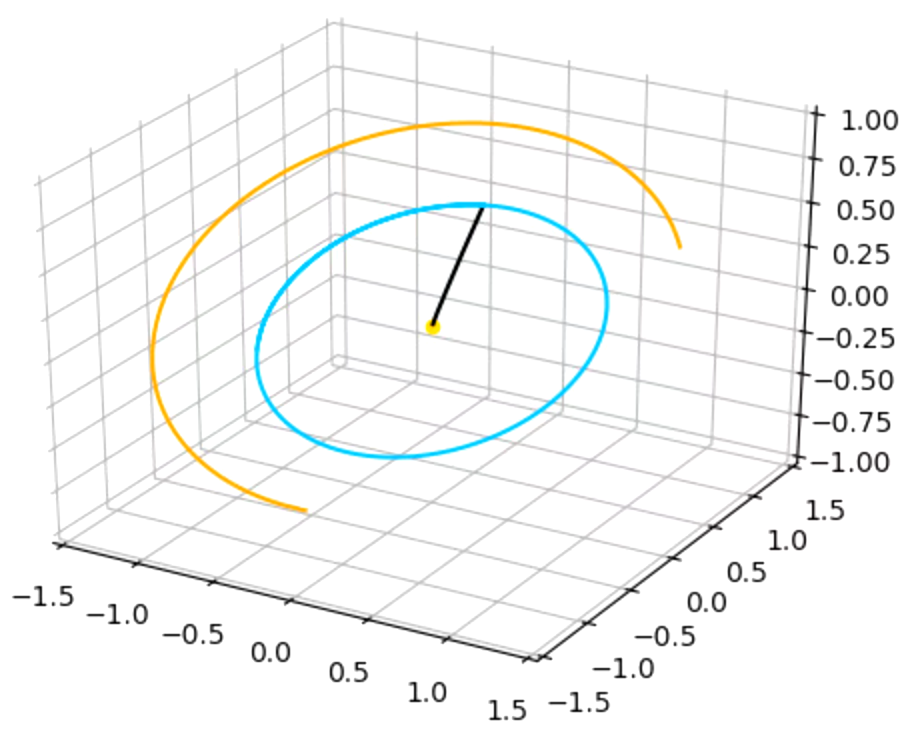
\includegraphics[width=0.50\linewidth]{fig/r4b-bug.png}
    \caption{3D plot of an early buggy 3D simulator. The yellow dot in the middle marks the Sun, Earth's orbit is traced in blue, Mars orbit in Red and the spacecraft trajectory traced in black. Instead of staying in orbit around the Earth, the spacecraft accelerated hard towards the sun in the very first time step iteration, crashing the program after 1473 iterations, just before reaching the sun faster than the speed of light.}
    \label{fig:r4b-bug}
\end{figure}

\subsection{What is unit testing?}
Complex computer software usually undergo various kinds of testing in its development cycle. For a computer program such as ours with lots of implemented mathematical formulae, the most relevant kind of systematic testing is \emph{unit testing}. In unit testing, various units of code are tested in isolation against some ``ground truth'', i.e. some test values that are obtained externally or manually written up. The units are often, as in our case, the \emph{functions} of the program. 

\subsection{Our Mathematica-Python Unit Testing Workflow and Why It Works}
Our simulator program is written in the Python programming language, most of it inside functions. For example, we have a function that iterates a single coordinate or momentum a single time step forward, a function that converts positions or velocity vectors between different coordinate system, and a function that calculates circular orbital speed or period.

The whole point of doing this is that \textbf{Mathematica provides nice visual formatting that allows mathematical equations to be pretty much identical to the complicated mathematical formulae written in hand or LaTeX}. Thus we can easily visually compare the implemented equations in Mathematica and in handwriting / LaTeX, and see that they match up. To give an example, here in \cref{fig:unit-testing-sympletic-euler-step-python-1,fig:unit-testing-sympletic-euler-step-python-2} is the implementation of the \texttt{} function in Python:

\begin{figure}[H]
    \centering
    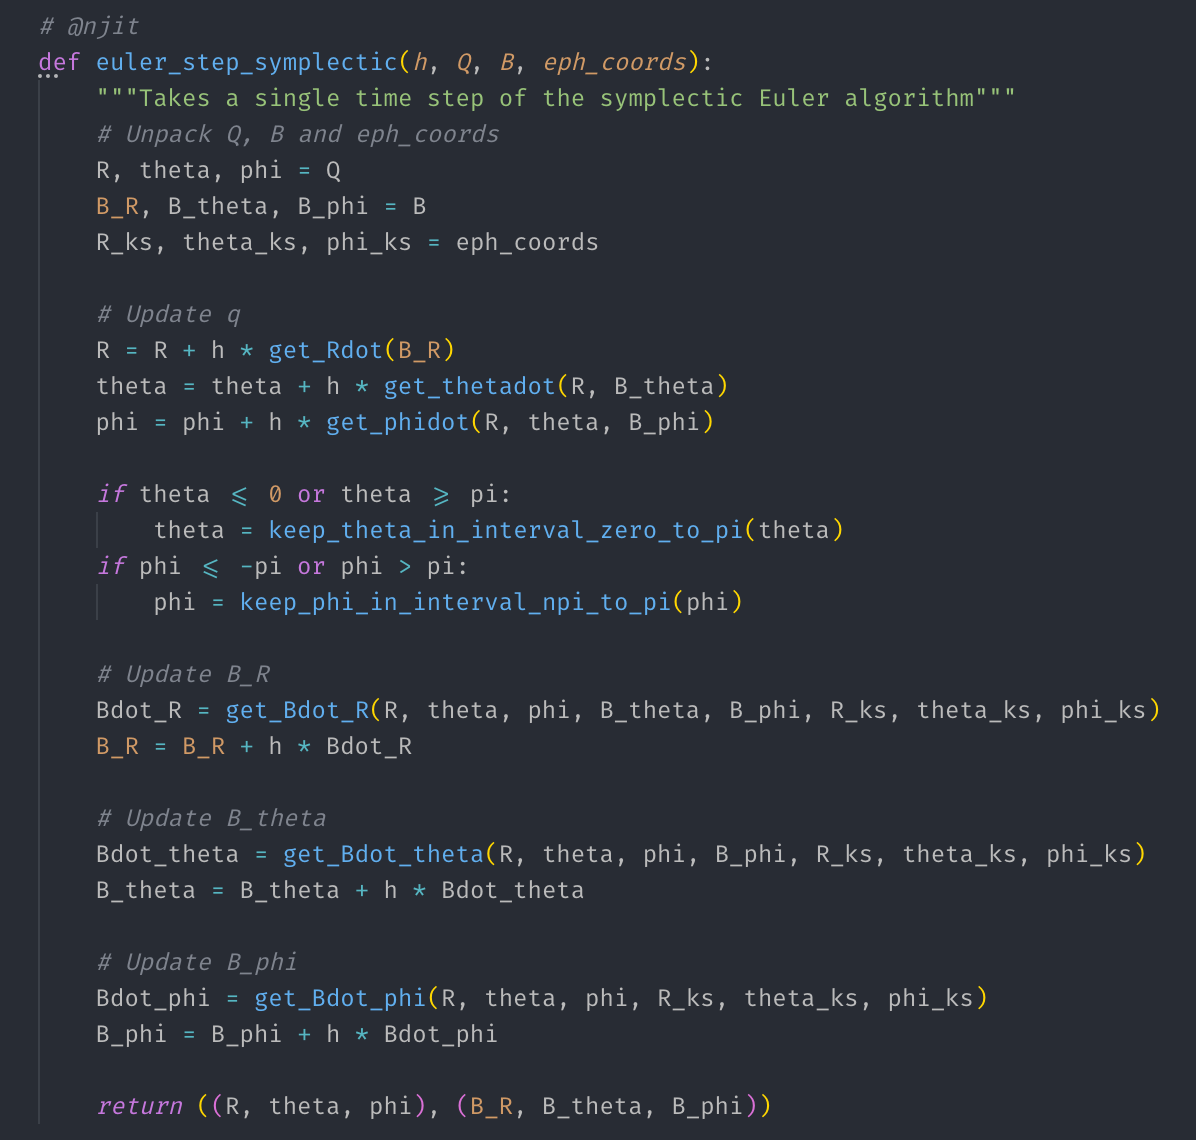
\includegraphics[width=0.90\linewidth]{fig/unit-testing-sympletic-euler-step-python-1.png}
    \caption{The main function of \texttt{symplectic\_euler\_step()} in Python.}
    \label{fig:unit-testing-sympletic-euler-step-python-1}
\end{figure}

\begin{figure}[H]
    \centering
    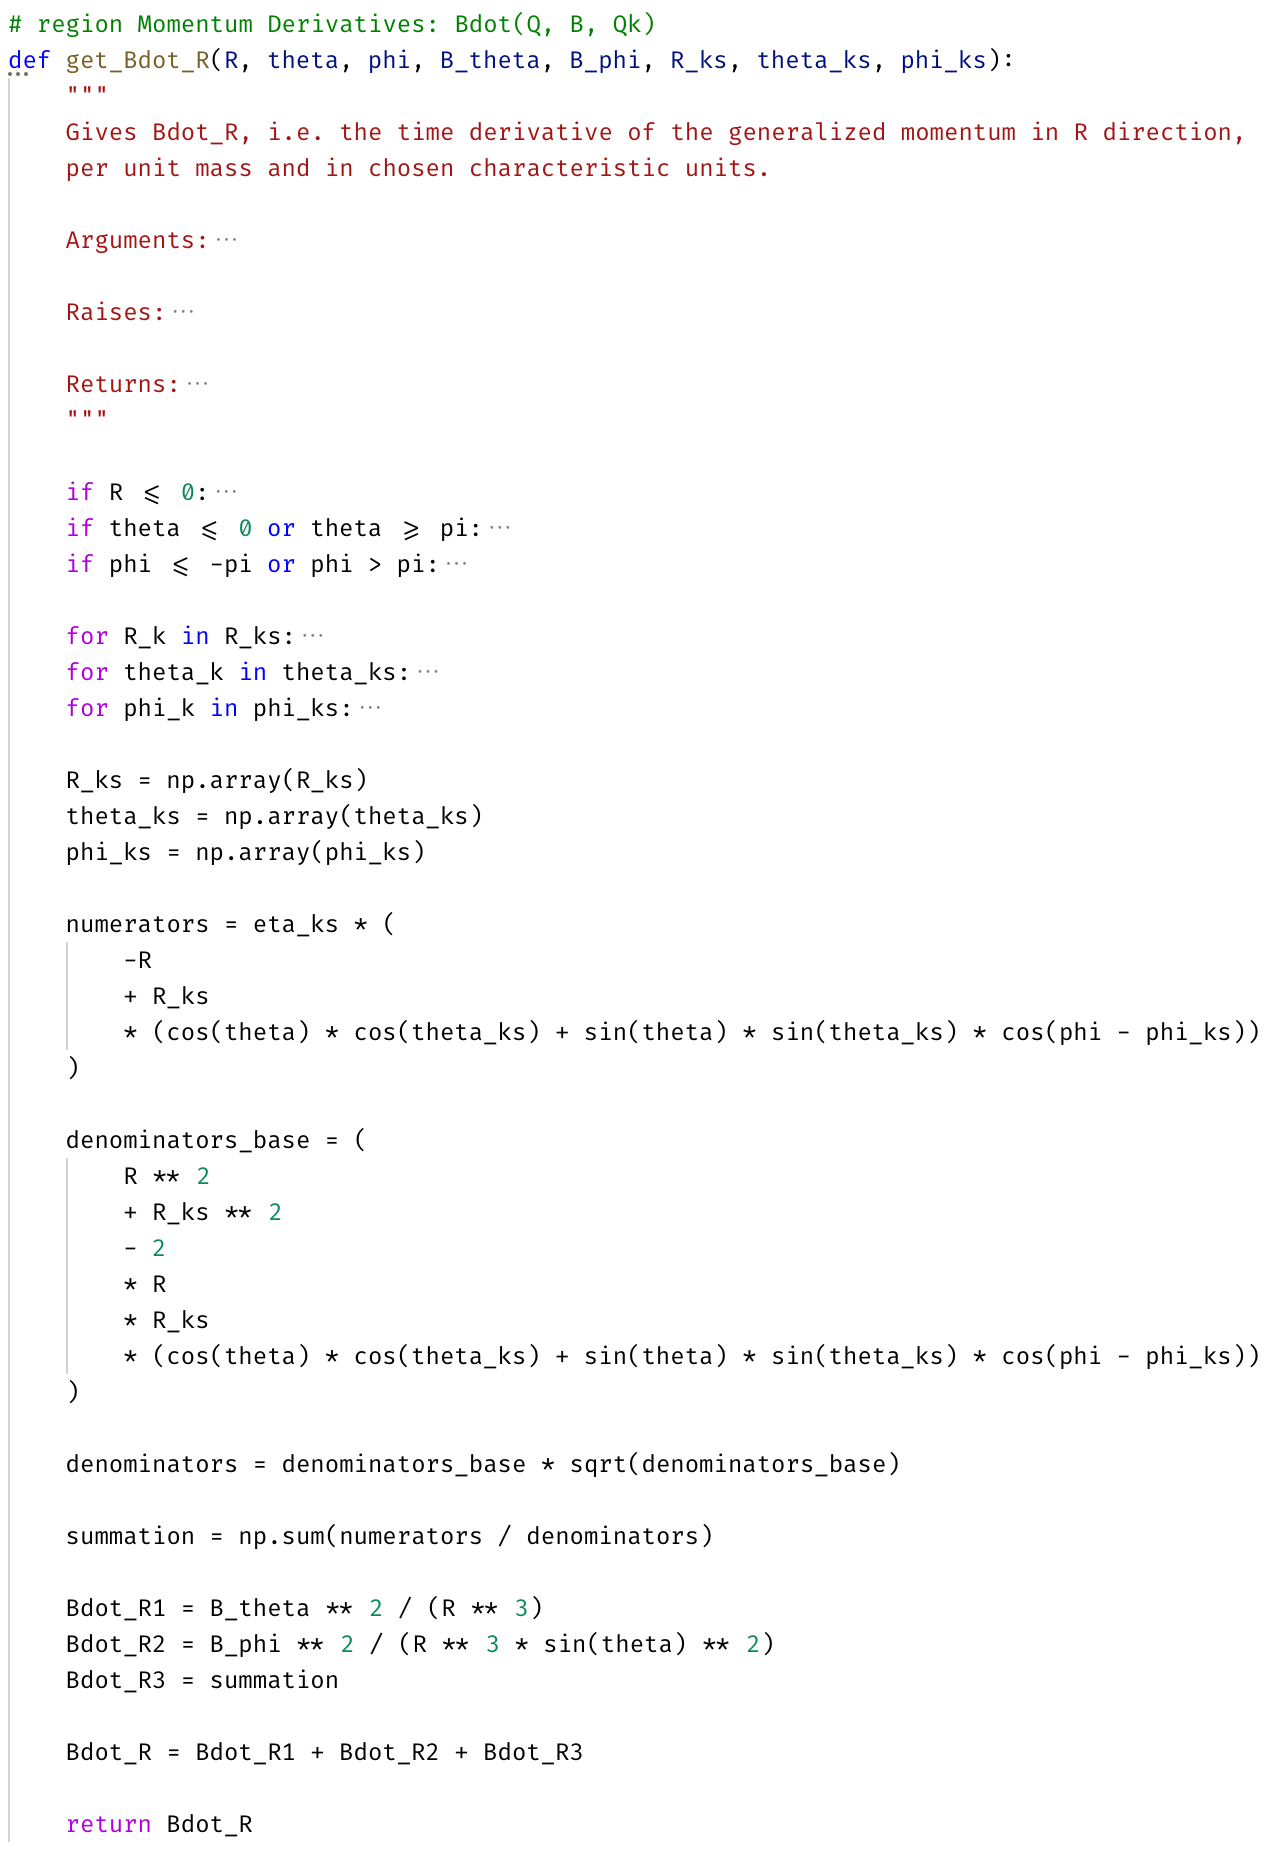
\includegraphics[width=0.90\linewidth]{fig/unit-testing-sympletic-euler-step-python-2.png}
    \caption{Function \texttt{get\_Bdot\_R(), which is just one of the sub-routines of \texttt{symplectic\_euler\_step()}}, in Python.}
    \label{fig:unit-testing-sympletic-euler-step-python-2}
\end{figure}

And here in \cref{fig:unit-testing-sympletic-euler-step-mathematica} is the same function in Mathematica:

\begin{figure}[H]
    \centering
    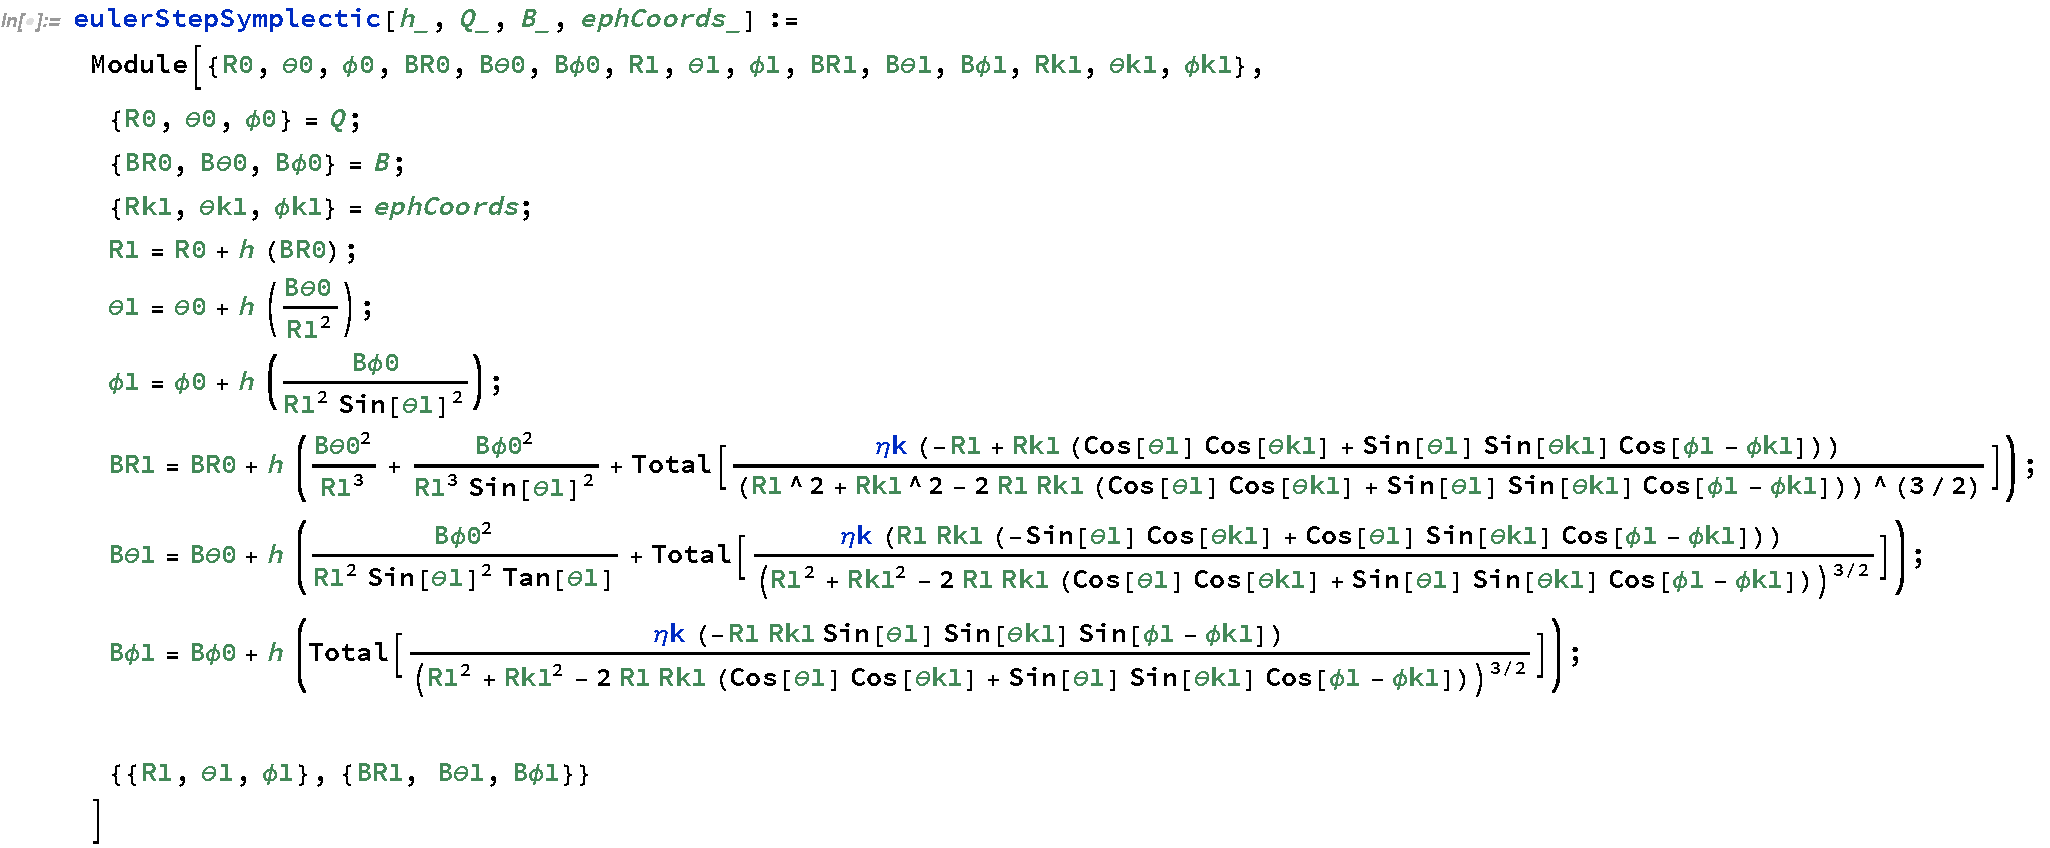
\includegraphics[width=1.0\linewidth]{fig/unit-testing-sympletic-euler-step-mathematica.pdf}
    \caption{The same function \texttt{symplecticEulerStep()} in Mathematica, which is obviously way more compact and readable than the Python counterpart.}
    \label{fig:unit-testing-sympletic-euler-step-mathematica}
\end{figure}

The point of comparison of \cref{fig:unit-testing-sympletic-euler-step-python-1,fig:unit-testing-sympletic-euler-step-python-2,fig:unit-testing-sympletic-euler-step-mathematica} above is that \emph{compactness} and \emph{readability} of the Mathematica version, thanks in large part to the 2D input syntax; Mathematica is simply a language built for handling mathematics really well. On the other hand, Mathematica doesn't scale well to larger and more complicated programs, performing on GPUs, using version control etc., where Python excels. But it does mean that Mathematica is a great application for testing your Python code – or rather providing test values that the Python code can be tested up against.

\subsection{The Python-Mathematica Testing Workflow}

The testing workflow can be described as such:

\begin{enumerate}
	\item \textbf{Write some piece of functionality as a function in Python.} It could be a mathematical formula, algorithm or just data-processing function.
	\item \textbf{Re-implement the same functionality Mathematica.} Ideally, one can use a built-in function if possible, such as when converting between spherical coordinates and cartesian coordinates. The benefit of Mathematica over Python is the aforementioned 2D display of input, which makes mathematical expressions much more compact and readable compared to Python code.
	\item \textbf{Export the test results (JSON) of various pairs of input/output.} Depending on the function a list of input can be a mix of random input, interesting edge-case input and invalid input. For functions with many input arguments, Mathematica can vary each input according to a list of numbers, and then generate all possible combinations of input arguments. \texttt{JSON} stands for JavaScript Object Notation, and is a standard file format for storing structured data. In this case, we used it for storing pairs of input and output for various functions.
	\item \textbf{Import test results (JSON) in python test script.} We used a Python test framework called pytest to set up automated tests that imported test data, and ran the test ``Output from Python-version-of-function(input) == Output from Mathematica-version-of-function(input)''.
	\item \textbf{Run tests using pytest and Coverage.py}. Coverage.py is a tool for measuring \emph{code coverage} of our Python program, meaning it can show what parts of the code is executed during running of all unit tests, both percentage-wise on an overall level, on file level and even line-by-line within code files, see \cref{fig:Coverage-py,fig:Coverage-py-file}. This was useful for systematically ensuring that all critical parts of the 3D simulator had been tested, and allowed everyone to directly see the progress in the debugging process.
\end{enumerate}


\begin{figure}[ht]
    \centering
    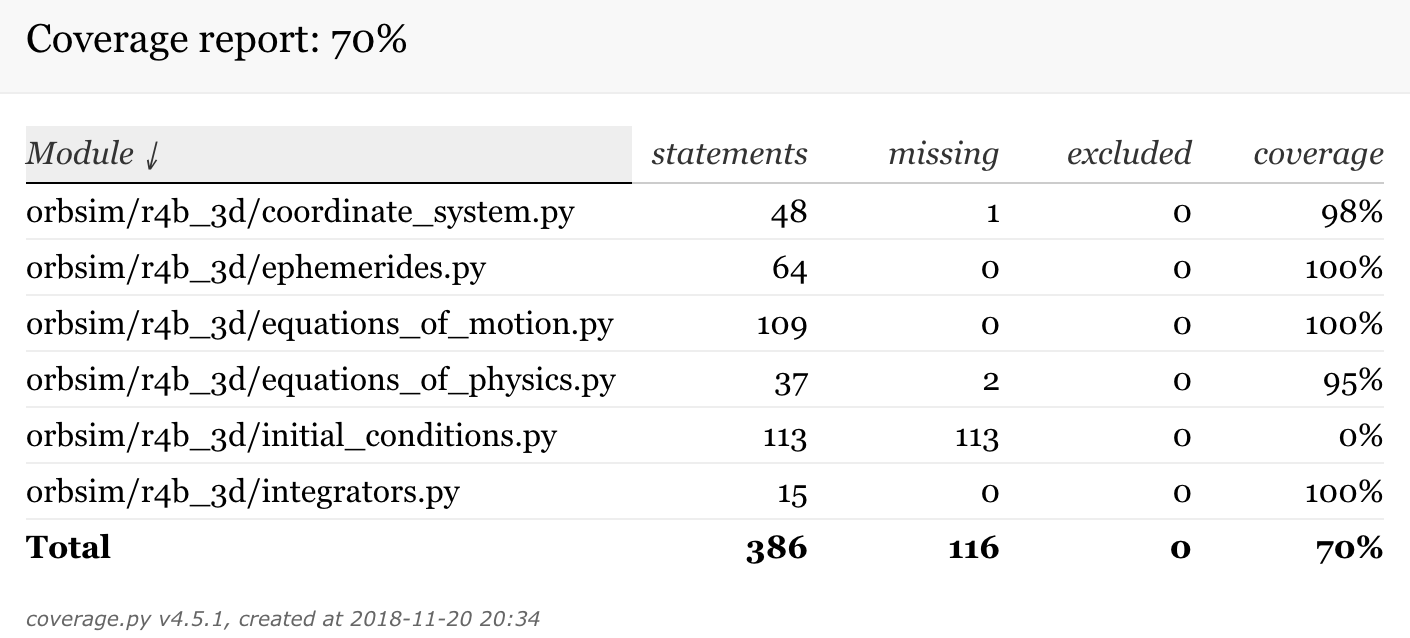
\includegraphics[width=0.90\linewidth]{fig/Coverage-py.png}
    \caption{Coverage.py generates a HTML file showing the \emph{code coverage} of the testing suite on a subset of the code. When we reached 70\% coverage, we were satisfied with the degree of certain of correctness of the critical parts of the code, and could verify that the 3D simulator now game the expected results in various scenarios, so we stopped testing then.}
    \label{fig:Coverage-py}
\end{figure}

\begin{figure}[ht]
    \centering
    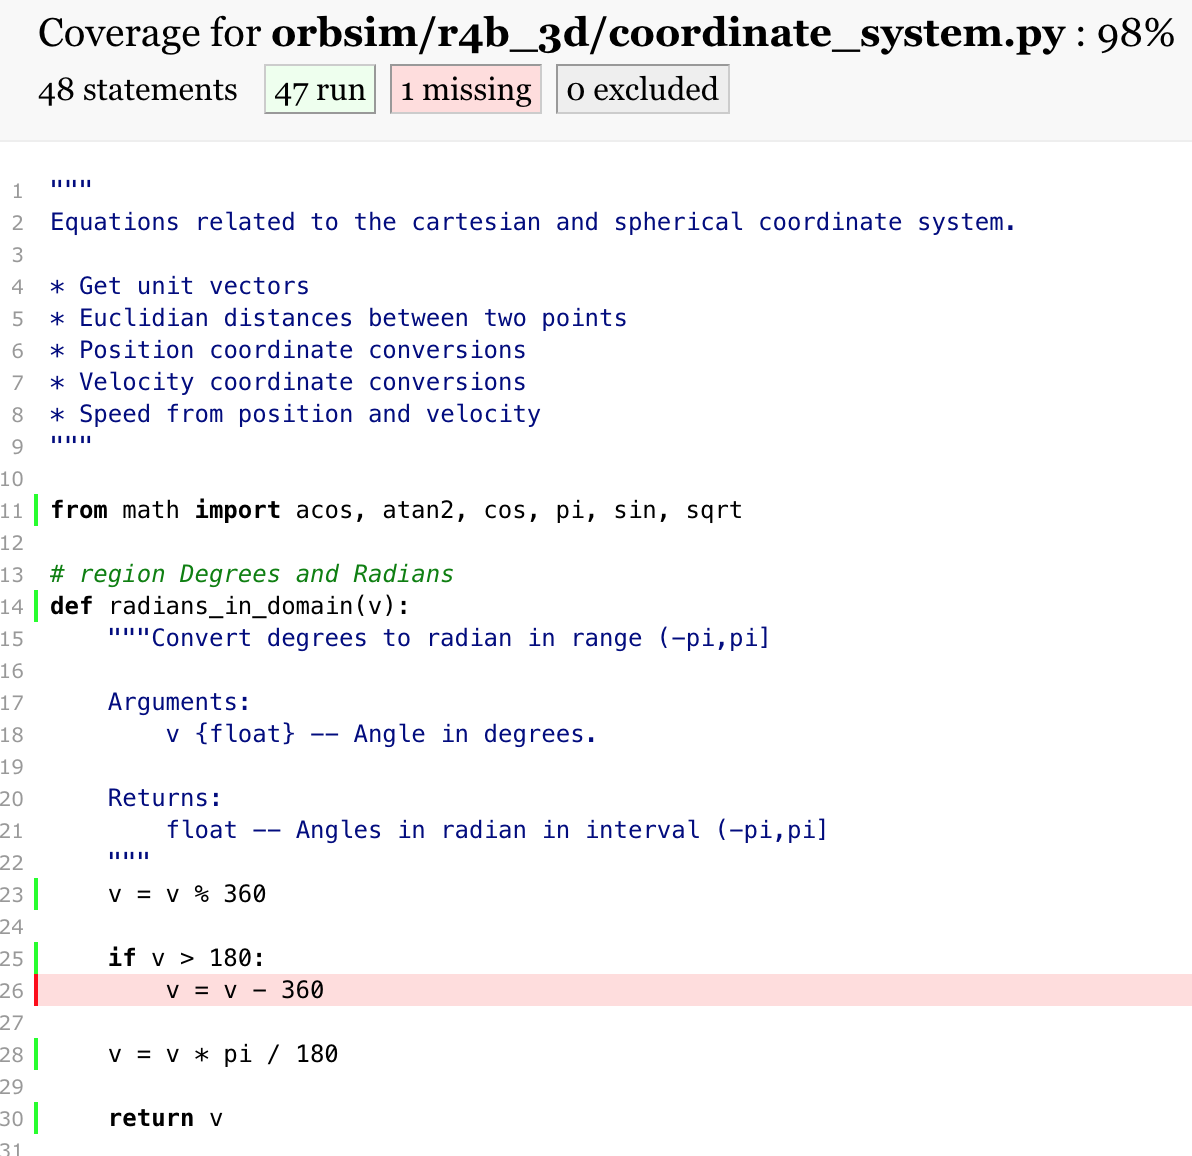
\includegraphics[width=0.90\linewidth]{fig/Coverage-py-file.png}
    \caption{Clicking a file shown in previous \cref{fig:Coverage-py} shows details of which lines have test coverage in the given file. Here, no test covers the case of $v > 180$ in the function $\texttt{radians\_in\_domain().}$}
    \label{fig:Coverage-py-file}
\end{figure}

During the debugging process we found a $+$-sign and $*$-sign that was mixed up, and a parenthesis that was closed at the wrong place, but was syntactically correct. Following this, the 3D simulator started to work as expected during basic tests of closed circular orbits etc.